\chapter{Introduction}

Inductive Functional Programming (IFP) is the automatic synthesis of declarative programs from an incomplete specification, typically given as pairs of Input-Output examples. Whilst this field has existed since the 1970s, recent work has slowed due to limitations on the complexity and structure of programs that can be learned. \\ \\
Answer Set Programming is a relatively new approach to logic programming, which works by computing the so called "Answer Sets" of a logic program which correspond the minimal models of that program. ASP has the advantage over traditional logic programming languages (i.e Prolog) that it is much more expressive, 

\section{Motivation}

My project introduces a new approach to IFP, through the use of ASP. Being oriented towards difficult search problems, ASP has been successfully applied to similar problems in the fields of planning, robotics and ontologies. Since one approach to IFP categorises the learning problem as a search problem over the range of possible programs, it seemed natural to apply ASP in this area. \\ \\
This project is does not just develop a new approach to IFP, but makes one that is easier to use as well. As they are developed by academics, existing IFP are either lacking user interfaces or have rudimentary ones, often making usage or translating results difficult. Through exploring ways to make the UI easier to use, it becomes possible to start considering possible application of this technology. \\ \\
I focused my project as a learning tool. It is not uncommon for a new Haskell student to be unfamiliar with recursion, having no experience in writing programs in a functional style. An easy to use IFP system could help beginners by allowing them to experiment with creating different programs, helping them become more familiar with the Haskell syntax.

\section{Contributions}

These motivations are achieved through the implementation of my tool. I have created a learning system consisting of a responsive, user-friendly web based user interface, a core learning algorithm based on ASP and a back end system used to communicate between the two. This system takes a set of input / output examples and uses these examples to subsequently learn and return a valid Haskell function. \\

\begin{figure}[h!]
\centering
\includegraphics[width=0.8\textwidth]{C1/structure.png}
\caption{Basic tool structure}
\end{figure}
\mbox{}\\
My ASP learning algorithm implements two different approaches. The first, detailed in Chapters 3 and 4, makes use of a Haskell interpreter implemented in ASP which runs Haskell programs re-written as ASP rules. This interpreter is then used in the learning task to determine which possible functions return the correct result when ran on the example inputs. The most optimal of these functions is returned as the learned result. \\ \\
The second approach, detailed in Chapter 5, maintains an ``equality constraint'' for each input example pair. This constraint is initialised with the fact that the result of a function call with a specific input should be equal to the respective output. Then, the constraint is maintained as the function call is evaluated, and fails if an obvious contradiction is reached (i.e. 1 = 2). Functions which do not fail this constraint over all input examples are returned as possible solutions.\\ \\
\begin{figure}[h!]
\centering
\includegraphics[width=0.5\textwidth]{C1/expression_tree.png}
\caption{Expression tree for a simple expression}
\end{figure}
\mbox{}\\
A second approach is necessary due to performance issues with the first approach. Using an interpreter means evaluating the value of all sub-expressions of a function, gradually combining expressions until an output is produced. This is inefficient as atoms have to be generated both when working out which expressions to evaluate, and when evaluating them. In comparison, the constraint-based approach fails as soon as a contradiction is reached, eliminating the need to produce an overall output to a function. \\ \\
The user interface is built to allow for easy experimentation and testing. Users can enter examples with any number of arguments, getting quick results in the form of the learned program. Then, if this program is incorrect the user can add a new counter-example or modify any examples that may be incorrect. In addition, if the user is unsure about a generated program then they can add examples with no respective output, which are then auto-completed. If the result of this auto completion is as expected, then the generated function is likely correct. \\ \\
\begin{figure}[h!]
\centering
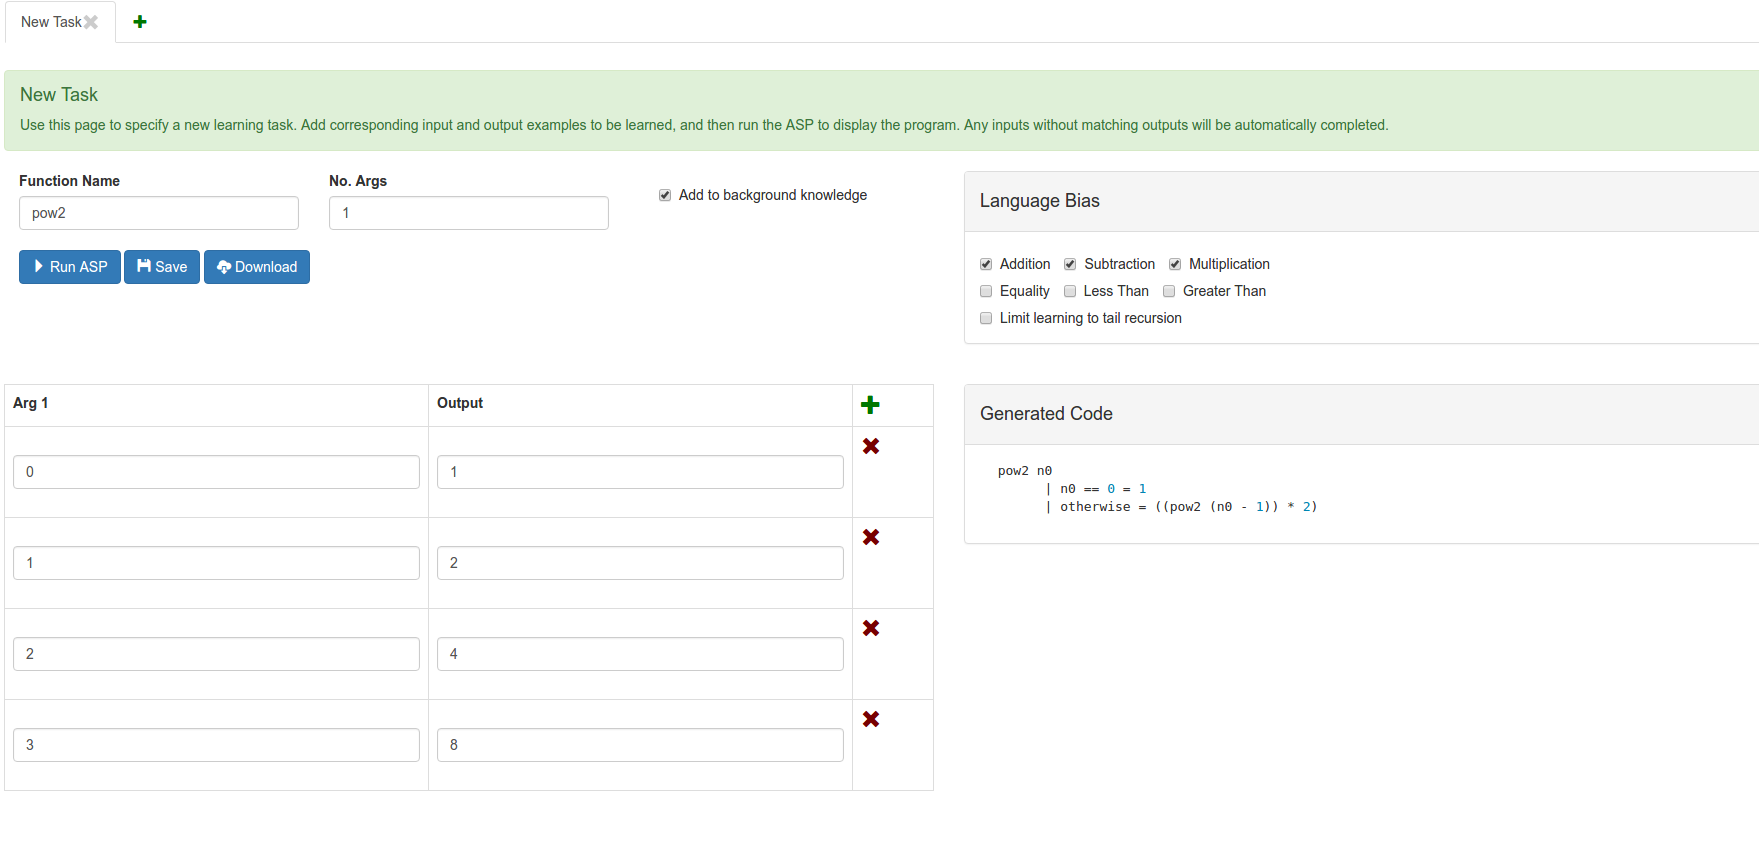
\includegraphics[width=\textwidth]{C1/screenshot_pow2.png}
\caption{Screenshot showing a simple example}
\end{figure}
\mbox{}\\
Consider the example seen in Figure 1.3, which details a simple program which calculates $2^n$. Given the input examples :\\
\begin{lstlisting}
Input : 0, Output : 1
Input : 1, Output : 2
Input : 2, Output : 4
Input : 3, Output : 8
\end{lstlisting}
\mbox{}\\
These examples then learn the Haskell program \\
\begin{lstlisting}
pow2 n
   | n == 0 = 1
   | otherwise = pow(n - 1) * 2
\end{lstlisting}
\mbox{}\\

\begin{figure}[h!]
\centering
\includegraphics[width=0.6\textwidth]{C5/project_workflow.png}
\caption{The iterative learning workflow}
\end{figure}
\mbox{}\\ 
The frontend is then linked to the algorithm by a backend written in Java. This backend manages all parts of the learning that would be too difficult to implement in either the frontend or the ASP, including :
\begin{itemize}
\item Generating skeleton rules enumerating all possible programs.
\item Converting inputs into valid ASP.
\item Running the learning task in parallel.
\item Converting the output from ASP rules to valid Haskell.
\item Running the generated Haskell to auto-complete empty examples.
\end{itemize}
\mbox{}\\
To evaluate the tool, I have ran various examples and recorded how each performs, on both approaches. The results, detailed in Chapter 7, have shown that the constraint based approach is on average 50\% faster than the interpreted approach. However, these results have also shown that the constraint based approach is less expressive than the interpreted one, having a more limited range of learnable programs.


\pagebreak
%\addcontentsline{toc}{section}{References}
%\renewcommand\bibname{{References}}
%\bibliography{References}
%\bibliographystyle{plain}